\chapter{Methodology}
\label{ch:method}

\section{Data warehouse}
To get the relevant data for solving this problem I first had to approach the wider problem of developing a robust data warehouse I started by building a dynamic data stream that could take data from an external source and store it in the company data warehouse so I would be able to run new iterations of the model as new data came in. To facilitate the problem of having a dynamic data import stream I used the python object relation mapping library since it has direct support for the python data library pandas . Doing this allows me to read data in any supported format and store it in a SQL database with the correct data types. The data I need is stored in an Amazon S3 bucket, so I used the python S3 library Boto3 to read TSV files from blob storage every hour and stored them in the data warehouse. I then deployed this process onto a docker container using the Azure cloud tool called Container Instances that enables docker containers to run as scheduled tasks. Docker containers are standardised units of software that contain all of the dependencies for running a specific program or script in a single executable package which can be run in the cloud or on a local machine.

\section{CRISP-DM Methodology}

As previously mentioned, I am going to be using the CRISP-DM model (\cite{Wirth2000CRISP-DMMining}) to break down the problem into 6 specific stages \textbf{reference the figure from intro} 

\section{Business Understanding}

This section asks what the company requires and hopes to gain from the process; in this case, the company requires a better understanding of which customers are most likely to cancel their reservations. This will helps in not only preventing cancellations but also in gaining a better understanding of why cancellations occur. Understanding why bookings are being cancelled through the process of feature and model explanation is also important from a machine learning and business perspective, as this will help to understand what the best actions are to prevent cancellations.

\begin{figure}[hbt!]
 %\centering
 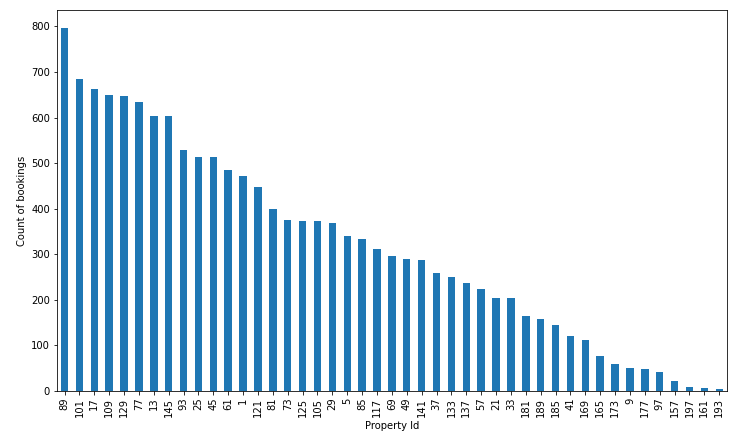
\includegraphics[width=10cm]{figures/bookings_by_property.png}
 \caption{The X axis shows each of the property Ids with the Y axis showing the total number of bookings made}
\end{figure}


The dataset contains 45 properties in total, with the number of students at each one varying significantly. Because of the large variation, it will be best to understand cancellations at the global level, with one model trained on data from all properties, as shown in figure 3.1. This helps to avoid model overfitting, as creating an accurate model with a small number of data points on some of the properties would be difficult. The risk here is that some of the discrepancies between the individual properties will go unnoticed by the model.

\section{Data Understanding}

The relevant booking data for this problem is created in an external system, which is the customer-facing website where each booking is taken. Customer information is stored in external website databases when a booking is made through the website. Personal information about the customer, such as name, address, date of birth, and phone number, is included in this data. As the customer progresses through the booking process, they will be directed to a page where they will be asked which university they will be attending and to select the property they wish to rent. The location of the property, the name of the room, the price, and any extras are all stored here. When a student chooses a room, they will be asked about the payment structure they prefer and how they plan to make their deposit. All of the relevant cost data is kept in this folder. In some cases, the fields for data entry in the booking system are not required, implying that the data will not be saved; in these cases, the value of the attribute is replaced with something else.

\vspace{5mm}

The information stored during these stages of the booking describes all of the intellectual property stored about each individual customer, and it is this information that will be used to forecast the customer's activity and whether or not they will cancel their reservation. In the case of a classification problem, any attribute that influences the target variable is relevant. Since the goal of machine learning is to collect as much useful data as possible

In this case I will be looking only at data from the years 2020 to 2021 since the historic data is incomplete. During this booking cycle there are a total of 14,363 bookings.

\begin{figure}[hbt!]
 %\centering
 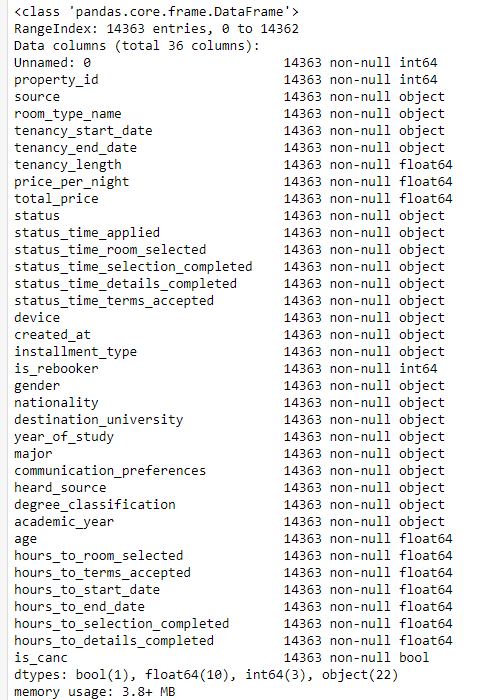
\includegraphics[width=10cm]{figures/df_info.png}
 \caption{Shows all of the attributes in the dataset}
\end{figure}

Figure 3.2 shows the features if the booking dataset. 

\begin{itemize}
    \item property id is the unique identifier for the residence 
    \item source is the internal system used to create the booking
    \item room type name is the category of room selected
    \item tenancy start date is the proposed start date of the contract
    \item tenancy end date is the proposed end date of the contract
    \item tenancy length is the duration in day the contract is valid for
    \item price per night is the daily rate at which the room will be sold
    \item total price is the total price for the contracted time
    \item status is the current status of the booking
    \item status time applied is the time the booking process was started
    \item status time room selected is the time the customer selected there room
    \item status time selection completed is the time the customer finalised the selected process 
    \item status time details completed is the time all personal details are entered
    \item status time terms accepted is the time the agreement is completed
    \item device is the type of the device the booking was made on
    \item created as is the time the process was started
    \item installment type is the payment schedule
    \item is rebooker defines if the same customer has applied before
    \item date of birth of the customer
    \item gender of the customer
    \item nationality of the customer
    \item destination university is the university the customer expects to go to
    \item year of study is the academic year  the customer is in
    \item major is the degree type of the student
    \item communication preference is the customer selected method of communication
    \item heard source is where the customer discovered the booking
    \item degree classification is the degree type of the customer
    \item academic year
\end{itemize}

\section{Data Preparation}

The dataset I have selected to be used for this research is a combination of 3 different tables from the external booking system, these include the booking table, student table and academic year id table. All of these tables have been combined from the data warehouse to create the DataFrame shown in \textbf{figure 3.7}. During the stage of feature selection I removed many of the attributes from these tables as I did not believe they would provide any value and did not contain good data quality. Using a dataset with too many columns has to potential to result in over fitting and noise in the model, it is possible that the dataset I have selected can be reduced to a smaller number of features but I believe I have selected the best dataset available to me for completing this research. 

\begin{figure}[H]
 %\centering
 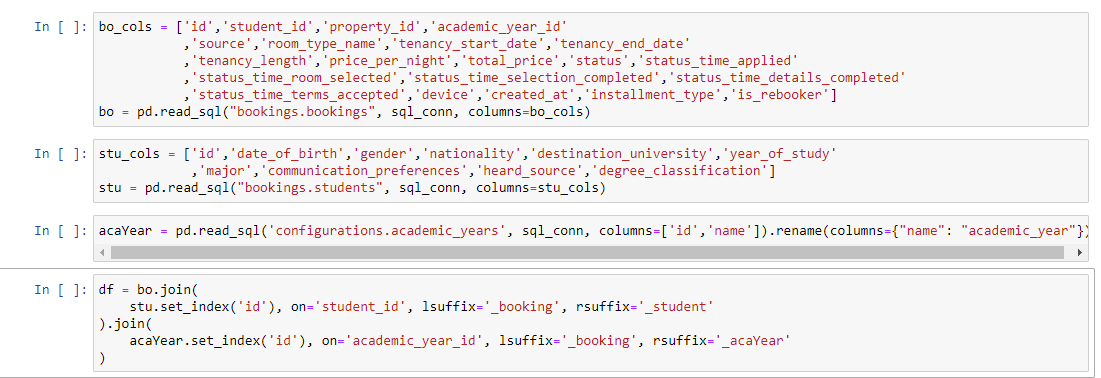
\includegraphics[width=10cm]{figures/joining_tables.png}
 \caption{Section of Jupiter Notebook for data cleaning where I joined 3 sql tables into 1 dataframe using there respective id's}
\end{figure}

With all of the necessary data stored in the data warehouse I imported the relevant tables into a Jupiter Notebook to perform the data cleaning stages. My aim is to include only valid bookings that made it the whole way through the booking process. I started by removing any booking in the dataset that didn't have a total price or with a total price less than 1 as this meant the booking was not stored in the system correctly and may have been used for testing. I then removed any booking that did not get to the terms accepted stage since this could not be treated as a cancellation or a booking as the customer process was not finished.

To account for the missing values in the categorical columns I use the pandas fill na method to replace the null values with 'Other'  to prevent errors from occurring during the modeling stages when trying to handle null values and to make it clear in the results when a missing value had been used.

\begin{figure}[H]
 %\centering
 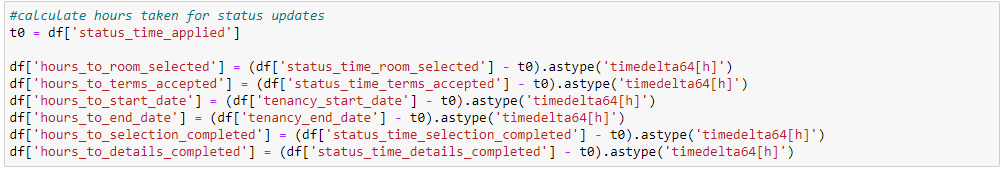
\includegraphics[width=10cm]{figures/time_variables.png}
 \caption{Section of Jupiter Notebook for data cleaning for feature engineering from the dataset by measuring the time taken to complete each stage of the booking process in the number of hours from the start date}
\end{figure}
Figure 3.5 shows the feature engineering I applied by using the status time applied column to act as the first point where the booking process was started. I created attributes used to store how long the customer took within each stage of the booking process as this describes the customers activity throughout the booking process, for example if a customer too only 1 hour to complete the booking process they may be less likely to cancel than one who too 2 days. 

Using the featurization auto setting allows Auto ML to automatically detect the column types and apply the optimal data preprocess techniques, for categorical data the One Hot encoding technique is applied to create a new variable for each stage of the categorical attribute represented as binary. The process of featurization is able to detect columns with high cardinality.  High cardinality means a attribute contains a large number of unique values, this was true for columns destination university, major and nationality this is an expected result as the dataset contains students from a large variety of university's and nationalities. When a feature with high cardinality is detected by Auto ML it is automatically dropped from the dataset. 

To handle missing numeric values imputation is applied by the automatic featurization in Auto ML by replacing any missing values with the average of the column. Imputing missing values working best in columns with only a small proportion of missing values, this is why I have dropped all columns with a significant proportion of missing values before this stage.

\section{Modeling}

I used Azure ML Studio to evaluate and compare multiple different algorithms. ML studio is a cloud environment used to train, deploy, automate, manage and track ML models. It can be used for multiple different types of machine learning like supervised or unsupervised and deep learning. It gives the ability to write code in Python, R and its own no-code environment.  I used the cloud Jupiter notebook features for the data cleaning and preparation stages as well as testing models. To evaluate and compare multiple different algorithms I used Automated ML through its Python SDK on my cleaned dataset. Doing this meant I was able to test a large variation of regression algorithms.

I used a train test split of 20 percent test size with the sklearn model selection library. 80 percent training data was used to ensure there was a sufficient amount of data to ensure good model accuracy. 

\begin{figure}[hbt!]
 %\centering
 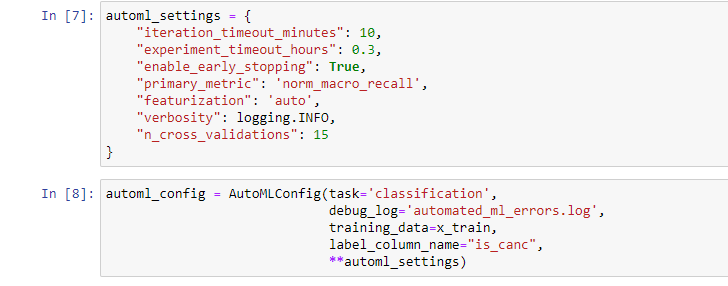
\includegraphics[width=10cm]{figures/auto_ml_settings.png}
 \caption{AutoML config settings for running classification algorithm}
\end{figure}

Running the algorithm is setup using the AutoMLConfig class in the Azure ML python SDK, the object contains all of the parameters used for configuring the experiment run. for a classification algorithm the task attribute is set to classification along with passing the training data and the target column label. Setting the number of cross validations to 15 means AutoML will run 15 different classifications on the training data outputting the results of each iteration. This output is then ranked by the selected primary metric which I have selected as norm macro recall, AutoML optimises models selected based on the primary metric. 

After the configuration is setup it can be passed to the Experiment.submit class, In this case I used the local run configuration so the cloud resources were not consumed running many iterations of the classification model. As each model is generated its results are outputted to the screen

\section{Evaluation}

The mode results will be evaluated based on the number of bookings accurately predicted as going to cancel, as this is the metric that best satisfies the problem specification. A successful model will be one that can classify over 50 percent of cancelled booking accuracy. This relatively low target accuracy is used because this is the first research completed in this specific field and therefore being able to accurately predict over 50 percent of canceled bookings shows that it is in fact possible to use a classification algorithm in predicting if a booking is going to be cancelled. Evaluating the CRISP-DM methodology needs to be concerned with understanding how each of the individual stages contributed to solving the final business objective. In most machine learning projects data understanding and data preparation have the most overall impact with a relatively small amount of time being taken in the modeling stage \cite{Polyzotis2018DataSurvey}. Evaluating how changes in the data being inputted into the model affects its ability to accurately predict cancellations.

\section{Deployment}

The deployment of the model will be handled by AutoML by registering the final model into the Azure cloud allowing it to then be accessed through the Azure API and integrated into any web supported system. The deployment of the model into the cloud is not within the scope of this project.



